% Top-level Evaluation chapter. \input this from the main manuscript.
% Requires in the preamble: \usepackage{booktabs} \usepackage{amsmath} \usepackage{amssymb} \usepackage{graphicx}
% If the main document uses a different graphics path for the figures, set it before \input.
\section{Experiments and Results}
\label{sec:eval}

We evaluate PCH, PI, and SPP (Section~\ref{subsec:privacy-objectives}) against a passive public-chain observer (Section~\ref{sec:eval-threat}).
The evidence comes from two attack families run on the same executions: a supervised attacker that tries to recover each hidden label from the on-chain observables, and an unsupervised attacker that asks whether the observables cluster along that label without seeing it.
Across the $45$ tasks, two meet the leakage criterion (one ICD-10 chapter and one nesting-depth contrast); both trace to the randomly drawn padding target, and the unsupervised attacker finds no natural grouping by the hidden labels beyond the same coincidence.
Table~\ref{tab:privacy-summary} summarizes the headline supervised verdicts across the three privacy objectives.
Beyond the privacy verdicts, we report the system's performance as a cost profile: per-transaction gas for commit and access (including the padding overhead), calldata sizes, circuit constraint count, and proving time, together with how circuit capacity, fixed-circuit policy complexity, and offline proof throughput scale.

% Sources of record (higher-AUC model per task; cross-checked against the JS verdicts):
%   PCH: python/results/supervised_analysis/pch_supervised_verdict.json
%   PI:  python/results/supervised_analysis/pi_supervised_verdict.json
%   SPP: python/results/supervised_analysis/spp_supervised_verdict.json
% (all 30 policy-disjoint seeds, deterministic per-seed RNG.)
% Dataset: Polygon Amoy, fixed circuit + commitment-only interface + access-gas padding.
\begin{table}[H]
  \centering
  \caption{Headline privacy results on the Polygon Amoy dataset. The supervised attacker
    uses 30 policy-disjoint seeds and a permutation test. A task passes unless both
    AUC$_{\text{mean}}>0.55$ and at least $50\%$ of seeds are significant.}
  \label{tab:privacy-summary}
  % Column widths sum to <1 so that the inter-column glue fits inside the text block.
  \begin{tabular}{p{0.16\linewidth}p{0.32\linewidth}p{0.42\linewidth}}
    \toprule
    Property & Hidden target & Headline supervised result \\
    \midrule
    PCH & DUO terms and ICD-10 chapters
        & 16 content-recovery tasks pass; DUO AUCs $0.493$--$0.526$, ICD AUCs $0.433$--$0.561$ \\
    PI & Related policy-pair identity
       & Overall AUC $0.514\pm0.022$, $7\%$ significant seeds \\
    SPP & Structure, predicate, parameter, and nesting-depth buckets
        & 28 pairwise contrasts pass; AUCs $0.483$--$0.629$, max $23\%$ significant seeds \\
    \bottomrule
  \end{tabular}
\end{table}

% Shared threat model for the three privacy experiments.
\subsection{Adversary and Observables}
\label{sec:eval-threat}

We consider the passive public-chain observer defined in Section~\ref{sec:problem}.
This adversary has unrestricted read access to the ledger and observes all transactions and events generated by TPS-ZKPI, but has no direct access to the plaintext policy or the witness.
Under the assumptions stated in Section~\ref{subsec:trust-model}, the zero-knowledge proof reveals no information beyond the public statement, and the hiding commitments conceal the committed policy.
These cryptographic protections do not, by themselves, prevent policy information from leaking through observable metadata.

We consider three adversary goals, one per privacy objective:
(i)~recover the policy's \emph{content} (PCH, Section~\ref{sec:eval-pch});
(ii)~distinguish two \emph{semantically related} policies (PI, Section~\ref{sec:eval-pi}); and
(iii)~recover the policy's \emph{structure or parameter sizes} (SPP, Section~\ref{sec:eval-spp}).

To evaluate attacks against these goals, we extract the following metadata features from each policy execution, consisting of a commit transaction followed by an access transaction:
%
\begin{itemize}
	\item \textbf{Gas:} \texttt{commitGasUsed}, \texttt{accessGasUsed}.
	\item \textbf{Calldata length:} \texttt{commitCalldataLength}, \texttt{accessCalldataLength}.
	\item \textbf{Proof size:} \texttt{proofSize}.
	\item \textbf{Event logs:} \texttt{commitLogsCount}, \texttt{commitLogsSize},
	      \texttt{accessLogsCount}, \texttt{accessLogsSize}.
\end{itemize}
%
The fixed circuit and commitment-only interface keep calldata length, proof size, and event-log counts and sizes constant across the evaluated policies.
These features remain in the attack pipeline but provide no variation for the attacks to exploit.
Any policy-dependent variation in the selected feature set must therefore occur in the two gas measurements (\texttt{commitGasUsed} and \texttt{accessGasUsed}).

% Shared methodology: supervised attack pipeline + unsupervised clustering cross-check.
\subsection{Attack Methodology}
\label{sec:eval-method}

We evaluate each privacy objective with a primary supervised attack and a complementary unsupervised cross-check.
The \emph{supervised} method trains classifiers on labeled data to predict hidden labels from the observables.
Performance is measured by AUC, with a chance baseline of $0.5$.
The \emph{unsupervised} method clusters the observables without using labels.
We evaluate agreement between the resulting clusters and the true labels using the Adjusted Rand Index (ARI) and Normalized Mutual Information (NMI).

We execute the generated policies on the \emph{Polygon~Amoy} testnet.
For each policy, a provider account submits the policy commitment using \texttt{commitPolicyWithGasPad}.
We then generate the Groth16 proof locally, acting as the TPS (Section~\ref{subsec:trust-model}).
A separate TPS account submits the access transaction using \texttt{requestAccessBoundWithGasPad}.
In the prototype, provider-to-TPS and requester-to-TPS exchanges are implemented as in-process calls and generate no additional on-chain artifacts.
We extract the observables defined in Section~\ref{sec:eval-threat} from the transaction receipts, calldata, and event logs.

\subsubsection{Supervised Attacks}
We evaluate each objective through binary classification \emph{tasks}, in which the attacker predicts a hidden label from the observables.
PCH tasks predict DUO-term presence or ICD-10 chapter membership (Section~\ref{sec:eval-pch}).
PI tasks distinguish between executions of two policies (Section~\ref{sec:eval-pi}).
SPP tasks distinguish between two categories of a structural or parameter property (Section~\ref{sec:eval-spp}).

For every task, we train two classifiers: logistic regression (LR) and random forest (RF), representing linear and non-linear models, respectively.
Each task is evaluated over \textbf{30 random seeds}, using the same protocol across PCH, PI, and SPP.

For each seed, we first randomly select one execution per policy to limit the influence of repeatedly executed policies on the AUC and its permutation test.
We then construct a \textbf{policy-disjoint $70/30$ train/test split}, ensuring that no policy appears in both sets.
Test AUC therefore measures attack performance on policies not seen during training.
Because policies are kept intact, exact per-class split proportions cannot always be achieved.
For each seed, we generate $512$ candidate splits and discard those that lack either class in the training or test set.
Among the valid candidates, we select the split that best approximates a $30\%$ test fraction within each class.

For each seed and classifier, we assess test AUC using a label-permutation test.
After training, we keep the test-set prediction scores fixed and randomly permute the test labels $R=500$ times.
We recompute AUC for each permutation to obtain its null distribution under no association between scores and labels.
The empirical $p$-value is
\begin{equation}
	p = \frac{k+1}{R+1},
	\label{eq:perm-p}
\end{equation}
where $k$ counts the permutations whose AUC is at least as large as the observed AUC.
The $+1$ correction prevents a zero $p$-value, with a minimum attainable value of $1/(R+1)$.
The result for a given seed and classifier is considered significant when $p<0.05$.

All tasks are binary, and the chance baseline for AUC is $0.5$ regardless of class balance.
Class imbalance may affect estimation uncertainty but does not change this baseline.

For each task, let $\mathrm{AUC}_s$ denote the test AUC for seed $s$, with $S=30$ seeds.
The results report the mean AUC and the AUC gap $G_{\mathrm{AUC}}$, defined as the mean absolute deviation from $0.5$:
\begin{equation}
	\mathrm{AUC}_{\text{mean}} = \frac{1}{S}\sum_{s=1}^{S}\mathrm{AUC}_s, \qquad
	G_{\mathrm{AUC}} = \frac{1}{S}\sum_{s=1}^{S}\left|\mathrm{AUC}_s-0.5\right|.
	\label{eq:auc-gap}
\end{equation}
Taking absolute deviations before averaging prevents values above and below $0.5$ from canceling.

The PASS/FAIL decision uses the mean AUC and the significant-seed fraction.
The latter is the fraction of seeds with $p<0.05$, reported as \%sig.
We classify each task as follows:
%
\begin{quote}
	\textbf{FAIL} if $\mathrm{AUC}_{\text{mean}}>0.55$ and at least $15$ of the $30$ seeds yield $p<0.05$.
	\textbf{PASS} otherwise.
\end{quote}
%
We refer to this rule as the \emph{leakage criterion}.
A PASS means that the evaluated attacks did not meet this criterion for the task.

The two conditions define an operational criterion based on effect size and consistency across splits.
With large test sets, even a small AUC increase above chance may be statistically significant.
The AUC threshold of $0.55$ prevents such small effects from triggering a FAIL solely on the basis of statistical significance.

The stability condition requires statistically significant results in at least half of the $30$ splits.
Because the splits overlap across seeds, the significant-seed fraction measures consistency across splits and is not interpreted as a combined $p$-value.

Because these thresholds are operational choices, we reapply the criterion over AUC thresholds of $0.52$--$0.60$ and significant-seed fractions of $0.3$--$0.7$.
At fractions of at least $0.5$, at most the two tasks discussed in the PCH and SPP result sections fail; lowering the fraction to $0.3$--$0.4$ adds at most two SPP contrasts, whereas raising it to $0.6$ yields none. No PI task fails under any of these threshold pairs.

In the evaluated run, the stability condition determines which tasks are flagged.
The AUC condition alone would flag four PCH and four SPP tasks.
In each objective, three of these tasks are significant in fewer than half of the splits.
The stability condition alone flags the same single task in each of PCH and SPP as the full leakage criterion.

In ten null reruns with policy-independent gas features, four contain a spurious PCH failure (a $3\%$ per-task frequency), while none produces an SPP failure.
We therefore examine the two observed failures in the corresponding result sections and keep them as FAIL.

The effectiveness of gas padding is assessed separately by the paired gas-padding ablation (Section~\ref{sec:eval-ablation}).
Using the same policies, features, splits, and classifiers, the attacks recover signal from the unpadded transcript, and that signal collapses after padding.
Thus, the leakage criterion summarizes residual attack performance, whereas the paired reduction provides the primary empirical evidence that padding suppresses the modeled gas channel.

The criterion is applied independently to LR and RF; a task fails if either classifier crosses both thresholds, and the result tables report the classifier with the higher mean AUC.

The classifiers receive all nine features stated in Section~\ref{sec:eval-threat}, including the seven that are constant by design.

\subsubsection{Unsupervised Clustering Attacks}
We run K-Means (with $K$ set to the number of classes, or $K=2$ for policy pairs) on the on-chain gas features, and score the recovered clusters against the true labels with ARI and NMI.
Values near $0$ mean the clusters carry no information about the hidden label; values near $1$ mean full leakage.

PCH clusters all executions globally, and SPP is clustered the same way on its $1{,}125$-execution view (Section~\ref{sec:eval-dataset}), once per annotation axis of Section~\ref{sec:eval-spp} with $K$ equal to that axis's bucket count.
At these sample sizes, ARI and NMI are read directly, each averaged over $20$ K-Means seeds.
To test whether an ARI exceeds chance, the cluster assignments are kept fixed, the labels are shuffled $200$ times, and $p_{\mathrm{ARI}}$ follows Equation~\eqref{eq:perm-p} with $R=200$, so its smallest attainable value is $1/201 \approx 0.005$.

For PI, clustering is scored per pair, so each side of a pair must contribute enough executions; this requires two safeguards.
First, the PI clustering analysis uses a dedicated set of \emph{balanced policy pairs} constructed from depth-layer executions (Section~\ref{sec:eval-dataset}).
We evaluate $127$ pairs, each containing $30$ executions per policy.
The policy pairs used in the supervised PI attack (Section~\ref{sec:eval-pi}) are unsuitable for per-pair clustering.
Most pairs contain only one execution per policy, while some contain $1$ execution for one policy and $30$ for the other.
These small or highly imbalanced samples make clustering scores unreliable indicators of policy distinguishability.
The supervised attack is unaffected, because it pools the executions of each pair type.
Second, NMI is \emph{permutation-debiased}. Even after balancing, each side of a pair holds only $30$ executions. At that scale NMI is inflated even without signal, whereas ARI is not (Section~\ref{sec:eval-nmi-sensitivity}), so ARI is read directly and NMI must be debiased.
The cluster assignments are computed once (K-Means does not see the labels) and the observed NMI is averaged over $20$ K-Means seeds; the pair labels are then shuffled $200$ times and the NMI recomputed against the fixed assignments on each shuffle, giving the null distribution of NMI under zero true signal.
The debiased NMI is the observed NMI minus the mean of this null distribution, and the empirical $p$-value $p_{\mathrm{NMI}}$ follows Equation~\eqref{eq:perm-p} with $R=200$, where $k$ counts the shuffles whose NMI meets or exceeds the observed value.
The cross-check flags a pair only if its debiased NMI is positive \emph{and} significant ($p_{\mathrm{NMI}}<0.05$).

% Dataset and corpus generation. \input from evaluation.tex after sec_threat_model.tex
% and before sec_methodology.tex. Numbers are of-record from
% experiments/data/polygonAmoy/executed_dataset.json and config.json (unpadded capture
% of 2026-10-15, v3.0.0-rc2 artifacts; see that directory's README.md).
\subsection{Dataset and Corpus Generation}
\label{sec:eval-dataset}

The PCH, PI, and SPP evaluations use policies from a dataset of $1{,}077$ distinct policies, run as $1{,}977$ on-chain executions on \emph{Polygon~Amoy}, each execution being one commit transaction followed by one access transaction.
The policies are produced by a deterministic generator with a fixed seed (\texttt{unified-decoupled-2026}), and the number of executions per policy follows from the two execution layers described below.
For reproducibility, the generator uses a deterministic test issuer to construct private credential witnesses for policies that require credential verification.

For each policy, the generator selects a set of DUO data-use terms and a logical form that combines them.
Five ontology-linked terms (Section~\ref{subsec:duo}) use code whitelists drawn from external vocabularies: DS uses ICD-10, RS uses the Ontology for Biomedical Investigations (OBI)~\cite{bandrowski2016ontology}, POA uses the Human Ancestry Ontology (HANCESTRO), GS uses ISO~3166 country codes, and CC uses SNOMED Clinical Terms (SNOMED~CT).
The other five terms (GRU, HMB, NMDS, GSO, NCU), which we call profile terms, are evaluated using signed claims from the requester's profile credential (Section~\ref{sec:design}).
The generator draws a fixed number of policies from each of six families defined by the terms and connectives they use: a single ontology-linked term, a single profile term, AND-only, OR-only, and mixed AND/OR combinations of several terms, and combinations of profile terms only.

Each policy contains one whitelist for each ontology-linked term it includes.
We draw a target whitelist size once per policy from $\{2, 4, 8, 12, 16, 20, 24, 32\}$, independently of its logical form.
This target applies to all whitelists in the policy.
If a selected scope contains fewer codes than the target, the corresponding whitelist contains only the available codes; this occurs in $8$ of the $2{,}000$ whitelists.
For analysis, we define a policy's whitelist size as the largest actual whitelist size within that policy.
The $147$ policies without an ontology-linked term are assigned a whitelist size of $0$.

For example, one generated policy combines the DUO terms RS (research-specific use) and DS (disease-specific use).
It requires the study design to belong to the OBI \emph{observational and comparative designs} family and the requested record to fall within the ICD-10 \emph{diseases of the circulatory system} chapter.
The two conditions are joined by \texttt{AND}, so access is granted only when both are satisfied.
Each condition is represented by a predicate that checks membership in a whitelist.
The RS predicate uses a whitelist of $8$ OBI study-design codes, while the DS predicate uses $8$ ICD-10 codes drawn from that chapter.
Both whitelist sizes fall within the ``medium'' parameter-size bucket in Table~\ref{tab:corpus}.

We execute the policies in two layers.
The \emph{coverage layer} executes $1{,}017$ distinct policies once each, spanning the content labels and the categories of policy structure and parameter size and allowing training and testing to use disjoint policies to assess generalization to unseen policies.
The \emph{depth layer} executes each of the $60$ policies in $30$ designed policy pairs $16$ times ($960$ executions), allowing training and testing to use different executions of the same policies to assess whether an observer can distinguish the policies within each pair.
For each request, the generator constructs requester evidence that either satisfies or violates the policy, so that the request is granted or denied.
In the coverage layer, granted and denied requests are balanced as closely as possible within each group of policies sharing a logical-form family and a set of DUO terms, to reduce associations between authorization outcomes and content labels.
Each depth-layer policy receives $8$ granted and $8$ denied requests.
All $1{,}977$ executions produced the planned authorization outcomes ($989$ granted and $988$ denied).

Every execution commits its own instance of its policy with fresh commitment randomness, so no two executions share a policy commitment, a parameter commitment, or an on-chain policy identifier.
The executions are submitted in an order shuffled with a fixed seed, independently of the policy labels, so the identifiers assigned in registration order carry no label information.
Every content label has at least $33$ policies, and Table~\ref{tab:corpus} summarizes the counts for each content label and each category of policy structure or parameter size.

% Source of record: experiments/data/polygonAmoy/executed_dataset.json (1077 policies,
%   1977 executions, generator seed "unified-decoupled-2026"; per-label policy and
%   execution counts: duoTermCodes, ontologyNamespace/ontologyValue, structureType,
%   nestingDepth, predicateCombo, paramType).
% DUO is multi-label: an execution carries every term its policy references, so the
% per-term rows overlap and their column sums exceed the corpus totals. ICD-10 rows
% cover only the policies with an ICD-10 scope (the DS policies), as the ICD-10 group
% heading states.
% Layout: groupings in pairs, side by side (DUO terms | ICD-10 chapters, then the SPP
% groupings two by two). Both label columns are as wide as and_or_mixed, so the two
% halves match. The empty 3em column 4 separates the halves; the rules under the group
% headings use \cmidrule without (l)/(r) trims, which latexdiff would break.
\begin{table}[htbp]
	\centering\footnotesize
	\caption{Composition of the shared policy corpus}
	\label{tab:corpus}
	\begin{tabular}{@{}w{l}{52pt}rr@{}w{l}{3em}@{}w{l}{52pt}rr@{}}
		\toprule
		Category      & Policies & Executions & & Category          & Policies & Executions \\
		\midrule
		\multicolumn{3}{@{}l@{}}{\textit{DUO data-use term} (multi-label)} & & \multicolumn{3}{@{}l@{}}{\textit{ICD-10 chapter} (DS policies)} \\
		\cmidrule{1-3}\cmidrule{5-7}
		GRU           & $302$    & $617$      & & ch0               & $44$     & $104$      \\
		DS            & $422$    & $677$      & & ch1               & $49$     & $94$       \\
		RS            & $412$    & $742$      & & ch2               & $33$     & $33$       \\
		POA           & $392$    & $737$      & & ch3               & $55$     & $100$       \\
		GS            & $382$    & $682$      & & ch4               & $41$     & $56$       \\
		CC            & $392$    & $632$      & & ch5               & $34$     & $49$       \\
		NCU           & $206$    & $506$      & & ch6               & $48$     & $63$      \\
		HMB           & $331$    & $661$      & & ch7               & $48$     & $48$       \\
		NMDS          & $237$    & $387$      & & ch8               & $33$     & $63$       \\
		GSO           & $236$    & $551$      & & ch9               & $37$     & $67$       \\
		              &          &            & & \textit{Subtotal} & $422$    & $677$      \\
		\addlinespace
		\multicolumn{3}{@{}l@{}}{\textit{SPP structureType}} & & \multicolumn{3}{@{}l@{}}{\textit{SPP nestingDepth}} \\
		\cmidrule{1-3}\cmidrule{5-7}
		trivial       & $130$    & $235$      & & flat              & $130$    & $235$      \\
		and\_only     & $294$    & $579$      & & shallow           & $210$    & $360$      \\
		or\_only      & $303$    & $513$      & & medium            & $335$    & $575$      \\
		and\_or\_mixed & $350$   & $650$      & & deep              & $402$    & $807$      \\
		\addlinespace
		\multicolumn{3}{@{}l@{}}{\textit{SPP predicateCombo}} & & \multicolumn{3}{@{}l@{}}{\textit{SPP paramType}} \\
		\cmidrule{1-3}\cmidrule{5-7}
		single        & $257$    & $497$      & & none              & $147$    & $297$      \\
		few           & $645$    & $1185$     & & small             & $232$    & $457$      \\
		many          & $175$    & $295$      & & medium            & $352$    & $547$      \\
		              &          &            & & large             & $346$    & $676$      \\
		\midrule
		\textbf{Corpus total} & $\mathbf{1077}$ & $\mathbf{1977}$ & & & & \\
		\bottomrule
	\end{tabular}

	\begin{tablenote}
		ICD-10 labels ch0--ch9 index the ten chapters used: A00--B99, C00--D48, D50--D89, E00--E90, F01--F99, G00--G99, I00--I99, J00--J99, K00--K93, and M00--M99.
	\end{tablenote}
\end{table}


The evaluated content labels cover ten DUO data-use terms and ten ICD-10 chapters (Table~\ref{tab:corpus}).
Evaluating every DUO term and individual ICD-10 code would require a substantially larger on-chain dataset.
We therefore evaluate DUO-term presence and ICD-10 chapter membership.


% Policy Content Hiding section body.
\subsection{Policy Content Hiding (PCH)}
\label{sec:eval-pch}

\noindent\textbf{Property.} PCH requires that the public-chain observer cannot recover the \emph{content} of a policy---its DUO data-use terms or the ICD-10 disease codes it references---better than chance.

\noindent\textbf{Scope of the labels.} The attack targets the ten DUO data-use terms of the corpus---general research use (GRU), disease-specific research (DS), research-specific restrictions (RS), population origins or ancestry research (POA), geographical restriction (GS), clinical care use (CC), non-commercial use (NCU), health or medical or biomedical research (HMB), no methods development (NMDS), and genetic studies only (GSO)---and disease codes aggregated to the ten ICD-10 chapters. This label restriction, its statistical-power rationale, and why category-level granularity is a conservative choice are detailed in Section~\ref{sec:eval-dataset}.

\noindent\textbf{Supervised attack.} Each DUO term defines a one-vs-rest binary task, on which we run the multi-seed pipeline of Section~\ref{sec:eval-method}.
Table~\ref{tab:pch-terms} reports the per-term verdicts: every DUO task stays below the $0.55$ AUC line, with mean AUC between $0.477$ and $0.540$; significant-seed fractions run up to $23\%$ (GRU), short of the $50\%$ gate, and with the AUC leg unmet none approaches the failure criterion.
The same pipeline applied to the ten ICD-10 chapters (one-vs-rest over the ICD-bearing rows only, median test $n{=}127$ per chapter; Table~\ref{tab:pch-icd10}) passes nine chapters and fails one.
Chapters ch1, ch2, and ch4 sit just above the AUC line (mean AUC $0.558$--$0.570$) but reproduce in at most $23\%$ of seeds, so they are boundary cases rather than stable channels.
Chapter ch5 (diseases of the nervous system) meets both legs: mean AUC $0.667$ with $53\%$ of seeds significant.
We report it as a FAIL of the criterion and examine below what the classifier separates.

\noindent\textbf{What the ch5 classifier separates.} The two gas features are the only non-constant observables, and the access-gas measurement is itself the sum of two parts: the target that the TPS draws uniformly at random from the padding band for that execution (Section~\ref{sec:design}) and the gas that the padded call consumes beyond it, which on Amoy is a near-constant $4{,}661$--$4{,}750$ gas for all $1773$ executions.
The observer sees only the sum, but the capture log records every target, so we can ask how much of the separability survives once the target is subtracted.
None does.
Over all $20$ PCH tasks the rank-based AUC of the access gas coincides with the AUC of the target alone to three decimals, and the AUC of the residual (gas minus target) lies between $0.47$ and $0.52$; for ch5 the gas and target AUCs are both $0.601$ and the residual AUC is $0.472$.
The $34$ ch5 policies simply drew targets whose mean lies $33{,}000$ gas above that of the other $388$ ICD-bearing policies, a $3.2\sigma$ deviation for a uniform draw of that size; because each coverage-layer policy is executed once, the $30$ seeds resample the same $34$ fixed draws, which is why the deviation reproduces across seeds.
Rerunning the of-record protocol unchanged on the residual in place of the access gas gives mean AUC $0.556$ with $10\%$ significant seeds (logistic regression) and $0.561$ with $17\%$ (random forest), a PASS; rerunning it on the target alone reproduces the FAIL ($0.686$, $63\%$).
The padded gas therefore carries a policy-independent random draw that happened to correlate with one chapter in this corpus, not information about the chapter; Section~\ref{sec:eval-method} quantifies how often the criterion produces such a false positive.



% Policy Indistinguishability section body.
\subsection{Policy Indistinguishability (PI)}
\label{sec:eval-pi}

PI evaluates whether an observer can identify which of two semantically related policies governs a given execution.
We evaluate PI using $30$ designed policy pairs, divided into three types with $10$ pairs each:
\begin{itemize}
	\item \texttt{semantic\_equivalent}: The two policies share the same logical form, consisting of the same DUO terms and Boolean structure, but differ in predicate parameter values, such as whitelist codes.
	\item \texttt{weak\_equivalent}: The two policies share the same set of DUO terms but differ in Boolean structure.
	\item \texttt{controlled\_difference}: The two policies differ in their sets of DUO terms. For each $k \in \{0,1,2,3,4\}$, we include two pairs whose policies differ in exactly $k$ of the four SPP dimensions (Section~\ref{sec:eval-spp}).
\end{itemize}
Each policy belongs to one pair, and which of its two policies is $P_0$ and which is $P_1$ is drawn at random.

The attacker knows both policies in a pair and can execute each policy to obtain labeled training examples.
Given the on-chain observables of an execution, the attacker predicts whether it was governed by $P_0$ or $P_1$.
For each random seed and policy pair, we split the executions of each policy equally between training and testing, separately for granted and denied outcomes.
We train LR and RF on the training executions and evaluate each classifier using test AUC.
Each execution commits a separate policy instance (Section~\ref{sec:eval-dataset}), so training and test executions never share a commitment.

For each pair type and classifier, we first average the test AUCs across the $10$ pairs for each seed.
To assess significance, we construct a null distribution of this average by repeatedly permuting the test labels within each pair, recomputing each pair's AUC, and averaging across pairs.
This yields one mean AUC and one permutation $p$-value per seed.
We then apply the leakage criterion (Section~\ref{sec:eval-method}) using the AUC averaged over the $30$ seeds and the fraction of seeds with $p<0.05$.

All three pair types are classified as PASS (Table~\ref{tab:pi-pairs}).
The highest mean AUC, $0.549$ for \texttt{semantic\_equivalent} pairs with RF, remains below the $0.55$ threshold, with $20\%$ of seeds significant.

% Source of record: experiments/results/supervised/pi_supervised_verdict.json
%   (higher-mean-AUC model per pair type; cross-checked against the JS pi_report.json verdict).
% Policy Indistinguishability -- within-pair supervised attack, 30 seeds; each seed tests
% half of the executions of every (policy, outcome) cell of every pair.
% Criterion: FAIL iff AUC_mean > 0.55 AND significant-seed fraction >= 0.5 (perm alpha=0.05,
% labels permuted within pairs). All three pair types gate.
% AUC gap = mean over seeds of |AUC_s - 0.5| from models.<m>.perSeed.auc.
% Positive control: positiveControl.models (synthetic N(0,1) feature shifted by 0.75 on P1);
% the column shows the model with the higher control mean AUC.
\begin{table}[htbp]
	\caption{Policy Indistinguishability: within-pair supervised attack over 30 seeds, by
		policy-pair type (higher-mean-AUC classifier per type).}
	\label{tab:pi-pairs}
	\centering\footnotesize
	\begin{tabular}{lcccccc}
		\toprule
		Pair type              & Pairs & AUC (mean\,$\pm$\,std) & AUC gap (mean) & \%sig  & med $n$ & Control AUC (\%sig) \\
		\midrule
		semantic\_equivalent   & $10$  & $0.549 \pm 0.035$      & $0.052$        & $20\%$ & $160$   & $0.649$ ($93\%$)    \\
		weak\_equivalent       & $10$  & $0.520 \pm 0.045$      & $0.042$        & $7\%$  & $160$   & $0.611$ ($63\%$)    \\
		controlled\_difference & $10$  & $0.478 \pm 0.026$      & $0.028$        & $0\%$  & $160$   & $0.621$ ($87\%$)    \\
		\bottomrule
	\end{tabular}

	\begin{tablenote}
		med $n$: median test-set size over seeds, summed over the $10$ pairs of a type ($16$ of the $32$ executions of each pair). Control: the attack with one added synthetic feature drawn from a standard normal distribution and shifted by $0.75$ for $P_1$; shown for the classifier with the higher control mean AUC (LR for all three types).
	\end{tablenote}
\end{table}

% Structure & Parameter Privacy section body.
\subsection{Structure and Parameter Privacy (SPP)}
\label{sec:eval-spp}

To evaluate SPP, we annotate each policy along four dimensions that capture the structural and parametric properties described in Section~\ref{subsec:privacy-objectives}.
The four dimensions are logical structure type (\texttt{structureType}), predicate count (\texttt{predicateCombo}), parameter size (\texttt{paramType}), and nesting depth (\texttt{nestingDepth}).
Each dimension is divided into discrete categories or value ranges.
Specifically, \texttt{structureType} classifies the logical form joining the DUO terms (Section~\ref{sec:eval-dataset}) into four categories: \texttt{trivial} (a single term with no Boolean connective, e.g.\ policy logic \texttt{"DS"}), \texttt{and\_only}, \texttt{or\_only}, and \texttt{and\_or\_mixed}.
\texttt{predicateCombo} groups policies by predicate-namespace count into \texttt{single} ($1$), \texttt{few} ($2$--$3$), and \texttt{many} ($\ge 4$);
\texttt{paramType} groups policies by whitelist size into \texttt{none} (no whitelist), \texttt{small} ($1$--$4$), \texttt{medium} ($5$--$16$), and \texttt{large} ($\ge 17$);
\texttt{nestingDepth} groups policies by the maximum nesting depth of the normalized expression into \texttt{flat} ($\le 1$), \texttt{shallow} ($2$), \texttt{medium} ($3$), and \texttt{deep} ($\ge 4$).
In the normalized expression, each term is joined by AND to the predicate that checks it (e.g.\ \texttt{"DS"} becomes \texttt{(DS \& P[ICD10])}).
The policy counts for each category in the dataset are listed in Table~\ref{tab:corpus}.

Each pair of categories within a dimension defines a binary classification task.
Using the observables, the attacker predicts which of the two categories the executed policy belongs to.

Table~\ref{tab:spp-contrasts} reports the results for all pairwise classification tasks.
For most tasks, mean AUCs are close to the chance level of $0.5$, ranging from $0.490$ to $0.546$.
The \texttt{structureType} task \texttt{trivial}/\texttt{or\_only} and the \texttt{nestingDepth} task \texttt{flat}/\texttt{medium} both have a mean AUC of $0.559$.
Although these values exceed the $0.55$ threshold, their significant-seed fractions are $27\%$ and $37\%$, below the $50\%$ threshold, so all $21$ tasks are classified as PASS.

% Source of record: experiments/results/supervised/spp_supervised_verdict.json
%   (higher-AUC model per contrast; cross-checked against the JS report.json verdict).
% Structure & Parameter Privacy — supervised attack, multi-seed (30 policy-disjoint seeds).
% AUC is the higher of logistic regression / random forest per contrast (the
% "stronger attacker" leg used for gating).
% Criterion: FAIL iff AUC_mean > 0.55 AND significant-seed fraction >= 0.5 (perm alpha=0.05).
% structureType has a 5th category, "trivial": single-atom policies with no boolean
% connective (e.g. logicOriginal "GR" or "DS"), previously misclassified as and_only.
% p_perm and the AUC-gap std are not emitted by the Python pipeline; %sig (the gating
% significant-seed fraction) is retained, so the table now runs five columns.
\begin{table}[H]
  \caption{Structure \& Parameter Privacy: 28 pairwise contrasts across four annotation
    axes, each over 30 policy-disjoint seeds. AUC is the higher-scoring of logistic
    regression and random forest per contrast (the stronger-attacker classifier used for
    the verdict). Every contrast passes: the four contrasts whose AUC exceeds $0.55$---all
    separating the tiny \texttt{none}-predicate or \texttt{none}-parameter class from a
    populated one---reach at most $20\%$ significant seeds, far short of the $50\%$ gate.}
  \label{tab:spp-contrasts}
  \centering\footnotesize
  \begin{tabular}{lcccc}
    \toprule
    Contrast & AUC (mean\,$\pm$\,std) & AUC gap (mean) & \%sig & med $n$ \\
    \midrule
    \multicolumn{5}{l}{\textit{structureType}} \\
    trivial / or\_only                & $0.539 \pm 0.043$ & $0.042$ & $23\%$ & $156$ \\
    trivial / and\_only                & $0.535 \pm 0.044$ & $0.042$ & $3\%$  & $78$  \\
    trivial / negation\_heavy          & $0.508 \pm 0.046$ & $0.034$ & $3\%$  & $138$ \\
    trivial / and\_or\_mixed           & $0.533 \pm 0.047$ & $0.047$ & $13\%$ & $108$ \\
    and\_only / or\_only              & $0.531 \pm 0.050$ & $0.045$ & $10\%$ & $140$ \\
    or\_only / negation\_heavy        & $0.520 \pm 0.036$ & $0.033$ & $10\%$ & $202$ \\
    or\_only / and\_or\_mixed         & $0.489 \pm 0.026$ & $0.024$ & $0\%$  & $170$ \\
    and\_only / negation\_heavy       & $0.512 \pm 0.041$ & $0.035$ & $3\%$  & $125$ \\
    and\_only / and\_or\_mixed        & $0.513 \pm 0.059$ & $0.051$ & $0\%$  & $95$  \\
    negation\_heavy / and\_or\_mixed  & $0.516 \pm 0.044$ & $0.038$ & $7\%$  & $155$ \\
    \midrule
    \multicolumn{5}{l}{\textit{predicateCombo}} \\
    none / single   & $0.582 \pm 0.129$ & $0.130$ & $0\%$  & $74$  \\
    none / few      & $0.629 \pm 0.099$ & $0.138$ & $20\%$ & $216$ \\
    none / many     & $0.617 \pm 0.106$ & $0.119$ & $13\%$ & $59$  \\
    single / few    & $0.515 \pm 0.036$ & $0.031$ & $7\%$  & $284$ \\
    single / many   & $0.500 \pm 0.039$ & $0.029$ & $0\%$  & $127$ \\
    few / many      & $0.483 \pm 0.029$ & $0.026$ & $0\%$  & $269$ \\
    \midrule
    \multicolumn{5}{l}{\textit{paramType}} \\
    none / small    & $0.543 \pm 0.115$ & $0.096$ & $3\%$  & $66$  \\
    none / medium   & $0.612 \pm 0.080$ & $0.125$ & $17\%$ & $204$ \\
    none / large    & $0.545 \pm 0.093$ & $0.086$ & $0\%$  & $78$  \\
    small / medium  & $0.521 \pm 0.033$ & $0.030$ & $10\%$ & $263$ \\
    small / large   & $0.513 \pm 0.048$ & $0.036$ & $0\%$  & $138$ \\
    medium / large  & $0.486 \pm 0.023$ & $0.022$ & $0\%$  & $277$ \\
    \midrule
    \multicolumn{5}{l}{\textit{nestingDepth}} \\
    flat / shallow   & $0.522 \pm 0.040$ & $0.037$ & $13\%$ & $228$ \\
    flat / medium    & $0.499 \pm 0.043$ & $0.036$ & $3\%$  & $106$ \\
    flat / deep      & $0.490 \pm 0.033$ & $0.030$ & $0\%$  & $103$ \\
    shallow / medium & $0.511 \pm 0.028$ & $0.023$ & $0\%$  & $240$ \\
    shallow / deep   & $0.492 \pm 0.032$ & $0.026$ & $0\%$  & $237$ \\
    medium / deep    & $0.492 \pm 0.040$ & $0.032$ & $0\%$  & $115$ \\
    \bottomrule
  \end{tabular}
\end{table}

% Cross-objective unsupervised clustering section (consolidated view + PI rebalancing).
\subsection{Unsupervised Clustering: A Label-Free Cross-Check}
\label{sec:eval-clustering}
The clustering attacker stated in Section~\ref{sec:eval-method} tests whether the on-chain observables group by a hidden label without access to that label.
Table~\ref{tab:clustering-summary} summarizes the clustering results across the three privacy objectives.

ARI stays within $\pm 0.003$ for every PCH, PI, and SPP target except the SPP \texttt{nestingDepth}, indicating little agreement between the clusters and the hidden labels.
The PCH and SPP NMI values are below $0.03$, and apart from \texttt{nestingDepth} none is significant under the label-permutation test ($p_{\mathrm{NMI}}\ge 0.08$).
For PI, $6$ of the $127$ pairs ($5\%$) have $p_{\mathrm{NMI}}<0.05$, consistent with the nominal $5\%$ level.


For \texttt{nestingDepth}, the ARI and NMI are small but statistically significant under the label-permutation test reported in Table~\ref{tab:clustering-summary}.
To investigate this association, we repeat clustering on the same executions, retaining commit gas and replacing access gas with the residual defined in Equation~\eqref{eq:gas-decomp}.
The nesting-depth ARI then falls to $-0.0004$, and neither ARI nor NMI remains statistically significant ($p_{\mathrm{ARI}}=0.60$, $p_{\mathrm{NMI}}=0.69$).
Together with the diagnostic for the \texttt{medium}/\texttt{deep} contrast in Section~\ref{sec:eval-spp}, this result is consistent with a chance association between the randomly drawn padding targets and nesting depth in the evaluated dataset.
However, the residual analysis yields a small but nominally significant ARI for \texttt{paramType} ($0.0026$, $p_{\mathrm{ARI}}=0.04$), whose NMI is not significant ($p_{\mathrm{NMI}}=0.09$).
These findings provide complementary evidence to the supervised results on the same dataset.

% Sources of record:
%   PCH-DUO:   experiments/results/clustering/pch/pch_global_duo_clustering.csv
%              (global, all 1773 executions, no layering; K = 10 primary DUO terms)
%   PCH-ICD10: experiments/results/clustering/pch/pch_global_icd10_clustering.csv
%              (global, all 770 executions of the DS policies, which carry the ICD-10 scope; no layering)
%   PI:        experiments/results/clustering/pi/pi_balanced_debiased.csv
%              (127 balanced 30v30 pairs; observed means)
%   SPP:       experiments/results/clustering/spp/spp_clustering_summary.csv
%              (raw field names logicStructure/predicateCount/setSize map to the
%               supervised axes structureType/predicateCombo/paramType)
% Dataset: experiments/data/polygonAmoy/ (same executions as the supervised verdicts).
% p_ARI / p_NMI are the permutation p-values of the ensemble ARI / NMI (ari_p_value / nmi_p_value).
% Residual diagnostics (cited in sec_clustering.tex, not in this table):
%   experiments/results/supervised/pad_residual_diagnostic.json
%   experiments.spp.clustering.{nestingDepth,paramType}.residual
\begin{table}[htbp]
	\centering
	\caption{Unsupervised clustering attack (K-Means, $K$ = number of classes, $K=2$ for
		pairs) on the on-chain gas features.}
	\label{tab:clustering-summary}
	\footnotesize
	\setlength{\tabcolsep}{4pt}
	\begin{tabular}{@{}llcccccc@{}}
		\toprule
		Objective & Target                   & $n$    & \#cls. & ARI       & $p_{\mathrm{ARI}}$ & NMI      & $p_{\mathrm{NMI}}$ \\
		\midrule
		PCH       & DUO terms                & $1773$ & $10$   & $0.0000$  & $0.48$             & $0.0109$ & $0.41$             \\
		PCH       & ICD-10 chapters          & $770$  & $10$   & $0.0021$  & $0.06$             & $0.0281$ & $0.08$             \\
		PI        & policy pairs ($30$v$30$) & $127$  & $2$    & $0.0020$  & ---                & $0.0139$ & ---                \\
		SPP       & \texttt{structureType}   & $1125$ & $4$    & $0.0004$  & $0.33$             & $0.0034$ & $0.34$             \\
		SPP       & \texttt{predicateCombo}  & $1125$ & $3$    & $-0.0005$ & $0.58$             & $0.0015$ & $0.51$             \\
		SPP       & \texttt{paramType}       & $1125$ & $4$    & $-0.0000$ & $0.49$             & $0.0030$ & $0.43$             \\
		SPP       & \texttt{nestingDepth}    & $1125$ & $4$    & $0.0071$  & $<0.01$            & $0.0088$ & $<0.01$            \\
		\bottomrule
	\end{tabular}

	\begin{tablenote}
		For PI, ARI and NMI are means across the $127$ balanced policy pairs.
		Each pair is clustered and tested separately, so no single $p$-value applies to these means (---).
	\end{tablenote}
\end{table}



% Sample-size sensitivity of NMI under a null where all classes are i.i.d.
% Source of record: experiments/analysis/clustering/nmi_null_simulation.py (seed 20260923)
%   -> experiments/results/clustering/null/nmi_null_simulation.{json,md}; T=1000 per row.
% Supports the clustering cross-check (Section~\ref{sec:eval-clustering}): explains why
% small-sample NMI can be elevated even with no class-distinguishing signal.
\section{Sample-Size Sensitivity of NMI}
\label{app:nmi-sensitivity}

The clustering cross-check reads ARI directly but debiases the NMI of the balanced PI pairs (Section~\ref{sec:eval-method}).
To examine that choice, we quantify how \emph{finite-sample effects} alone can inflate NMI
even when there is \emph{no} discriminative signal, using an idealized null in which all
classes are statistically indistinguishable.

We sample every class from the \emph{same} distribution, $z_{i}\sim\mathcal{N}(0,I_{d})$ for all classes, where $I_d$ is the $d$-dimensional identity covariance and $d=2$ matches the two gas features the clustering uses.
Since no class carries class-specific information, a clustering algorithm should not recover class membership,
and both NMI and ARI should concentrate around $0$ as the sample size grows.

For each configuration we run $T=1000$ independent trials.
In each trial we
(i)~generate $G$ classes with $n$ i.i.d.\ samples per class from $\mathcal{N}(0,I_d)$, for $n_{\mathrm{tot}}=Gn$ samples in total, assigning each sample a class label by construction order (these labels are independent of the sample values, since all classes share one distribution),
(ii)~standardize the pooled data and apply K-Means with $K=G$ and ten initializations, as in the evaluation, and
(iii)~score the predicted assignments against these assigned class labels with NMI and ARI.
We vary $n$ while holding $G$ fixed, and report the trial means $\overline{\mathrm{NMI}}$ and $\overline{\mathrm{ARI}}$.
We consider a \textbf{PI-like} binary structure ($G=2$, $n\in\{3,10,50,100\}$), a five-class structure ($G=5$, $n\in\{3,10,100\}$), and a ten-class structure ($G=10$, $n\in\{3,10,77\}$) together with the observed ICD-10 chapter sizes ($49$--$135$ executions per chapter, $n_{\mathrm{tot}}=770$).

Table~\ref{tab:nmi-sample-size-sensitivity} shows that, although all classes are indistinguishable by construction, \textbf{NMI is noticeably positive at very small $n$ but collapses toward zero as $n$ grows}, whereas \textbf{ARI stays near zero throughout}.
For the binary structure, $\overline{\mathrm{NMI}}$ falls from $0.2074$ at $n=3$ ($n_{\mathrm{tot}}=6$) to $0.0420$ at $n=10$, and to $0.0072$/$0.0034$ at $n=50$/$100$.
The same trend holds with more classes, at a higher level for every $n$: with five classes $\overline{\mathrm{NMI}}$ goes from $0.4152$ ($n=3$) to $0.0102$ ($n=100$), and with ten classes from $0.5346$ ($n=3$) to $0.0239$ ($n=77$).
For the observed ICD-10 chapter sizes, a separate null run that averages each trial over $20$ K-Means seeds, as the evaluation does, gives a null NMI with mean $0.0246$ and $95$th percentile $0.0302$; the observed ICD-10 NMI of $0.0281$ is reached in $145$ of $1000$ null trials ($p=0.15$).

\begin{table}[htbp]
	\centering
	\caption{Sample-size sensitivity of NMI and ARI under the null hypothesis where all
		classes are i.i.d.\ sampled from $\mathcal{N}(0,I_d)$.}
	\label{tab:nmi-sample-size-sensitivity}
	\begin{tabular*}{0.54\linewidth}{@{\extracolsep{\fill}}rrrr@{}}
		\toprule
		$n$ (per class) & $n_{\mathrm{tot}}$ & $\overline{\mathrm{NMI}}$ & $\overline{\mathrm{ARI}}$ \\
		\midrule
		\multicolumn{4}{@{}l}{\textit{Two classes (as in a PI pair)}} \\
		$3$       & $6$   & $0.2074$ & $0.0127$  \\
		$10$      & $20$  & $0.0420$ & $0.0008$  \\
		$50$      & $100$ & $0.0072$ & $-0.0003$ \\
		$100$     & $200$ & $0.0034$ & $-0.0004$ \\
		\addlinespace
		\multicolumn{4}{@{}l}{\textit{Five classes}} \\
		$3$       & $15$  & $0.4152$ & $-0.0034$ \\
		$10$      & $50$  & $0.1226$ & $0.0003$  \\
		$100$     & $500$ & $0.0102$ & $-0.0000$ \\
		\addlinespace
		\multicolumn{4}{@{}l}{\textit{Ten classes (as the DUO and ICD-10 targets)}} \\
		$3$       & $30$  & $0.5346$ & $-0.0009$ \\
		$10$      & $100$ & $0.2087$ & $0.0003$  \\
		$77$      & $770$ & $0.0239$ & $-0.0001$ \\
		\addlinespace
		\multicolumn{4}{@{}l}{\textit{Ten classes, observed ICD-10 chapter sizes}} \\
		$49$--$135$ & $770$ & $0.0244$ & $-0.0001$ \\
		\bottomrule
	\end{tabular*}

	\begin{tablenote}
		$T=1000$ trials per row, one K-Means fit with ten initializations per trial; $n_{\mathrm{tot}}$ is the total sample size.
		For the observed ICD-10 chapter sizes, the text also reports a separate run that averages each trial over $20$ K-Means seeds, as the evaluation does.
	\end{tablenote}
\end{table}

% Gas-padding ablation / mechanism attribution.
\subsection{Gas-Padding Ablation}
\label{sec:eval-ablation}

Only the gas measurements vary across policies within the selected feature set (Section~\ref{sec:eval-threat}).
We therefore use the ablation to assess how randomized gas padding affects the attackers' ability to infer hidden policy information.

We compare two configurations, B1 and B2, that differ only in whether randomized gas padding is enabled.
Both use the fixed circuit, commitment-only interface, and TPS execution profile.
We evaluate both configurations on the same policy subset, selected deterministically from the evaluation corpus.
B1 disables padding for both policy commitment and access transactions, whereas B2 enables it for both.
B2 uses the same protection configuration as the PCH, PI, and SPP evaluations (Sections~\ref{sec:eval-pch}, \ref{sec:eval-pi}, and~\ref{sec:eval-spp}).

To quantify the effect of padding on attack performance, we compare the absolute AUC deviation from $0.5$ under B1 and B2.
For each paired train/test split $s$, we define
%
\begin{equation}
	\Delta_{\text{leak},s} =
	|\mathrm{AUC}_{\mathrm{B1},s} - 0.5| -
	|\mathrm{AUC}_{\mathrm{B2},s} - 0.5|,
	\label{eq:delta-leak}
\end{equation}
%
where positive values mean padding moved the attacker closer to chance.

For each task, we compute $\Delta_{\text{leak},s}$ over $30$ paired train/test splits, one for each random seed, using the same test policies for B1 and B2 in each split.
We report the mean $\Delta_{\text{leak}}$ with a $95\%$ percentile-bootstrap confidence interval (CI), obtained by resampling the split-level differences.
Table~\ref{tab:ablation-gas-padding} summarizes the results, and Figure~\ref{fig:ablation-paired} visualizes the comparison between B1 and B2.

% Source of record (supervised rows + counts):
%   python/results/supervised_analysis/gas_padding_supervised_deltaLeakage.csv
%   (metadata: gas_padding_supervised_metadata.json)
% B1 = unpadded gas transcript; B2 = deployed randomized access-gas padding.
% Effect = |AUC_B1-0.5| - |AUC_B2-0.5|; 95% repeated-split stability interval over
% 30 paired seeds (nonContemporaneous B1/B2 profiles).
% This table is ILLUSTRATIVE: the four supervised rows are representative contrasts whose
% stability interval of dLeak excludes zero (genuine reduction). They are NOT the full set.
% The full per-contrast distribution (all 49 rf + 49 lr contrasts, colored by dLeak CI
% sign) is the primary evidence and lives in Fig. fig:ablation-paired. Full-set counts:
%   RF: 36 reduce / 13 no-eff / 0 neg;  LR: 36 reduce / 11 no-eff / 2 neg.
% The unsupervised-ARI and gas-cost rows below are retained from the deployed on-chain
% ablation run (experiments/ablation/gas_padding/...); they are not part of the Python
% supervised recompute.
\begin{table}[H]
  \centering
  \caption{Gas-padding ablation on Polygon Amoy: representative contrasts illustrating the
    padding effect. B1 (no gas padding) and B2 (deployed, randomized access-gas padding) are
    aligned on the same policy set. Supervised AUC is the random-forest score (the stronger
    of the two classifiers here; see Section~\ref{sec:eval-method}); clustering reports K-Means ARI.
    $\Delta_{\text{leak}}>0$ (defined in the text) means padding moved the attacker toward chance,
    reported as the mean with a $95\%$ stability interval over $30$ paired splits. Each supervised
    row is, per experiment, the largest-signal contrast whose $\Delta_{\text{leak}}$ interval excludes
    zero (two for SPP), chosen to avoid cherry-picking. The full per-contrast distribution is in
    Figure~\ref{fig:ablation-paired}.}
  \label{tab:ablation-gas-padding}
  \begin{tabular}{lp{0.34\linewidth}cc}
    \toprule
    Attack & Target & B1 (unpad.) & B2 (pad.) \\
    \midrule
    \multicolumn{4}{l}{\textbf{Supervised} (RF AUC; $\Delta_{\text{leak}}$ with $95\%$ interval)} \\
    SPP   & \texttt{nestingDepth flat/deep}   & $0.847$ & $0.553$ \\
          & \quad $\Delta_{\text{leak}}=0.280$ CI$[0.254,0.304]$ & & \\
    SPP   & \texttt{structureType trivial/negation\_heavy} & $0.843$ & $0.524$ \\
          & \quad $\Delta_{\text{leak}}=0.276$ CI$[0.248,0.301]$ & & \\
    PCH   & ICD ch8                          & $0.918$ & $0.410$ \\
          & \quad $\Delta_{\text{leak}}=0.327$ CI$[0.302,0.349]$ & & \\
    PI    & \texttt{semantic\_equivalent}\,$^{\dagger}$  & $0.361$ & $0.500$ \\
          & \quad $\Delta_{\text{leak}}=0.140$ CI$[0.084,0.205]$ & & \\
    \midrule
    \multicolumn{4}{l}{\textbf{Unsupervised} (K-Means ARI)} \\
    PCH   & ICD-10 chapter                   & $0.064$ & $-0.005$ \\
    SPP   & logic structure                  & $0.043$ & $-0.001$ \\
    SPP   & predicate count                  & $0.054$ & $0.001$  \\
    \midrule
    \multicolumn{4}{l}{\textbf{Gas cost} (mean, B1 $\to$ B2)} \\
    \multicolumn{2}{l}{Commit gas} & $216{,}562$ & $303{,}556$ ($+40.2\%$) \\
    \multicolumn{2}{l}{Access gas} & $546{,}876$ & $753{,}310$ ($+37.7\%$) \\
    \bottomrule
  \end{tabular}

  \noindent{\footnotesize{$^{\dagger}$ B1 sits below $0.5$: the unpadded attacker separates the
  pair in the inverted direction (still $0.14$ from chance). $\Delta_{\text{leak}}$ is defined on
  $|\mathrm{AUC}-0.5|$.}}
\end{table}


Figure~\ref{fig:ablation-paired} shows each supervised task as one point, giving $20$ PCH, $21$ SPP, and $4$ PI tasks per panel.
The horizontal and vertical axes give the absolute deviation from $0.5$ of the mean AUC over the $30$ splits under B1 and B2, respectively.
A mean AUC below $0.5$ therefore also counts as a deviation.
Points below the diagonal indicate that padding moves the mean AUC closer to chance.
Both panels show the same pattern. Tasks with large deviations under B1 move well below the diagonal, whereas tasks near chance under B1 stay in the lower-left corner on both sides of the diagonal.

For RF, $21$ tasks have mean AUCs that deviate from $0.5$ by more than $0.15$ under B1.
Under B2, all $21$ fall below this level, and their median deviation is $0.037$, comparable to $0.041$ for the remaining $24$ tasks.
The confidence intervals for $\Delta_{\text{leak}}$ lie entirely above zero for all $21$ tasks, supporting a reduction in deviation from chance.
Across all tasks, the median deviation decreases from $0.137$ under B1 to $0.038$ under B2.
LR shows a similar pattern.
All $19$ tasks with deviations above $0.15$ under B1 fall below this level under B2, and the median deviation across all tasks decreases from $0.111$ to $0.037$.



Tasks already close to chance under B1 show no consistent change after padding.
For RF, $12$ tasks have CIs for $\Delta_{\text{leak}}$ that include zero, and their B1 deviations are at most $0.095$.
Another $6$ tasks have CIs entirely below zero, indicating increased deviation from chance, although their B1 deviations are at most $0.045$.
The largest increase occurs for ch5, whose mean AUC changes from $0.455$ under B1 to $0.631$ under B2.
Such increases may reflect chance associations between the randomly drawn padding targets and the hidden labels.
Related diagnostic analyses for ch5 and the \texttt{nestingDepth} comparison \texttt{medium}/\texttt{deep} illustrate this effect (Sections~\ref{sec:eval-pch} and~\ref{sec:eval-spp}).

\begin{figure}[htbp]
	\centering
	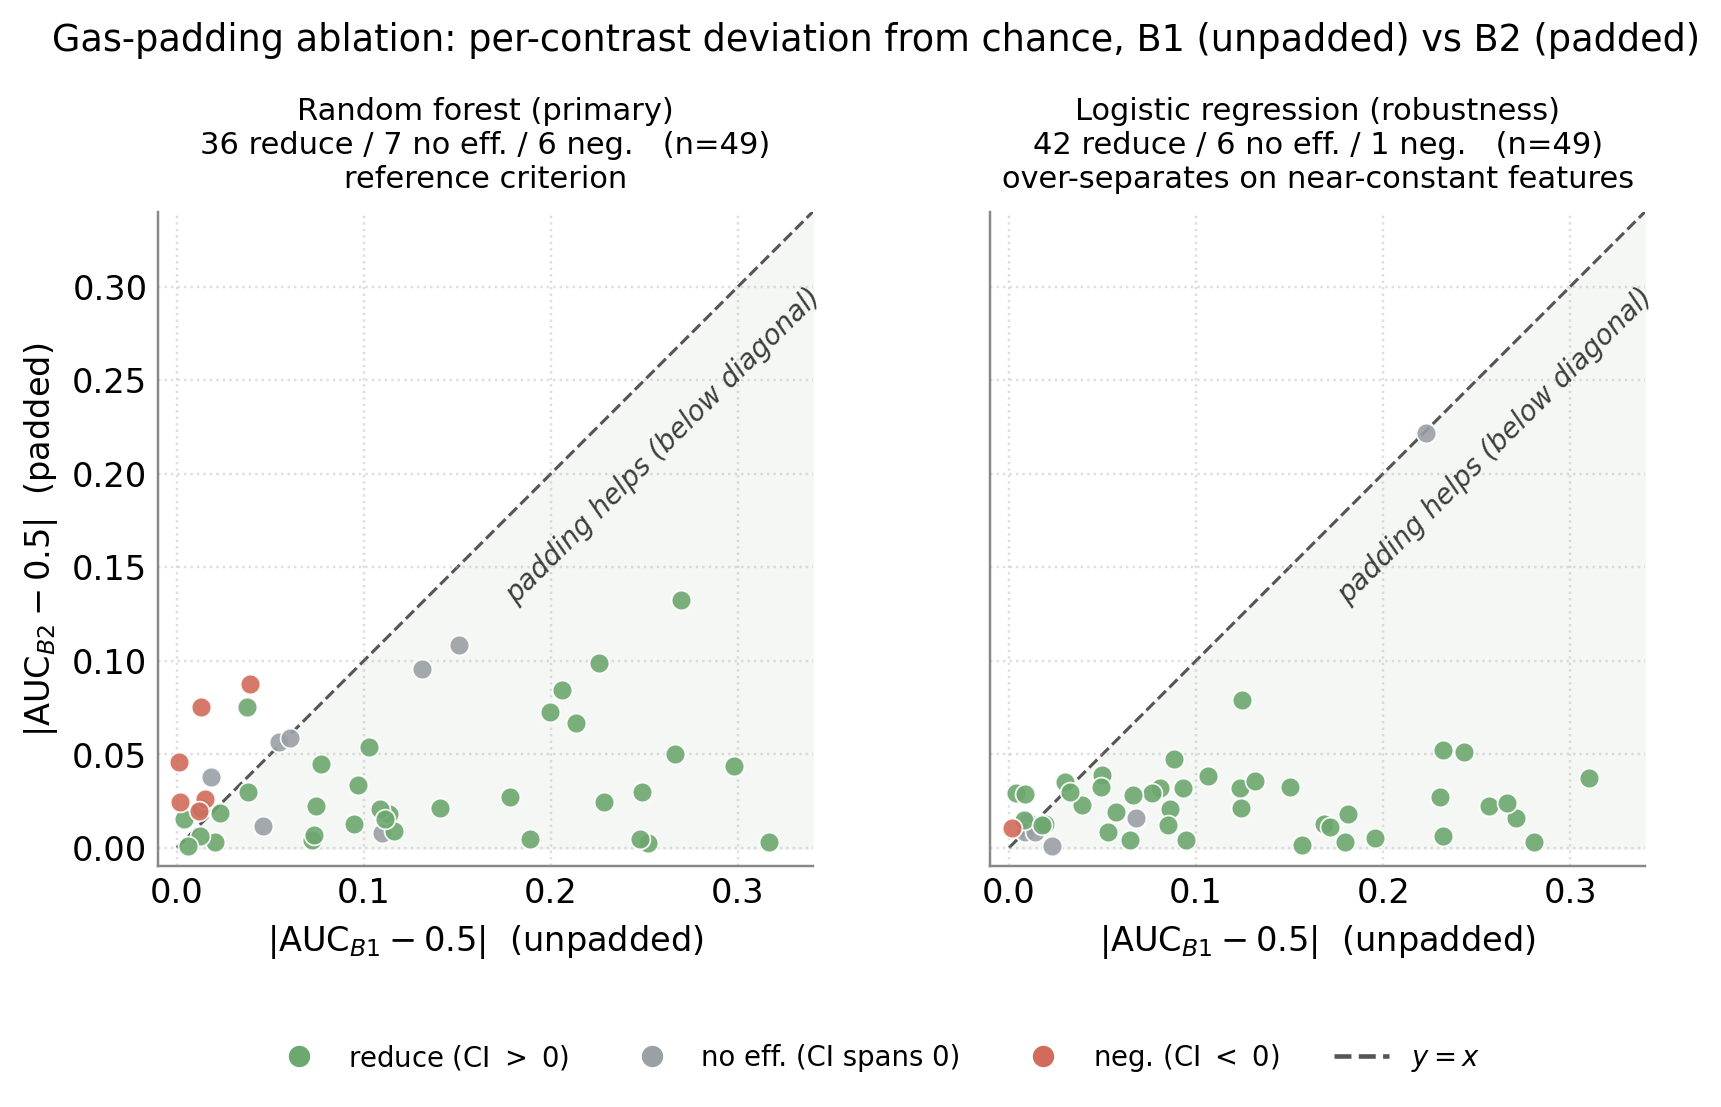
\includegraphics[width=\linewidth]{ablation_paired_scatter.png}
	\caption{Gas-padding ablation over the $45$ supervised tasks: (\textbf{a}) RF; (\textbf{b}) LR. Each point is one task, placed by the absolute deviation of its mean AUC from $0.5$ under B1 (horizontal axis) and B2 (vertical axis). Points below the dashed line $y=x$ moved closer to chance with padding. Blue, gray, and red points have $95\%$ CIs of $\Delta_{\text{leak}}$ above zero, spanning zero, and below zero, respectively.}
	\label{fig:ablation-paired}
\end{figure}

The clustering analysis provides complementary evidence.
Under B2, NMI decreases by $0.670$ for balanced PI pairs, $0.349$ for DUO terms, and $0.102$ for logical structure, with all three bootstrap confidence intervals excluding zero (Table~\ref{tab:ablation-gas-padding}).
With padding, NMI is at most $0.020$ for all three targets.

We next examine the source of the gas differences under B1.
Across the $1{,}119$ executions, unpadded access gas ranges from $723{,}288$ to $723{,}564$, excluding the first cold-start call.
Calldata analysis identifies two main sources of label-correlated variation arising from zero- and non-zero-byte pricing~\cite{akhunov2019eip2028}.
Different requester-pseudonym encodings produce an observed $192$-gas gap associated with profile-predicate use.
Sequential policy and resource identifiers introduce a further $24$-gas difference correlated with logical structure because policies were committed in groups by logical form.

Padding compensates for these calldata-pricing differences by bringing transaction gas consumption to the sampled target.
The remaining overhead varies by less than $100$ gas (Section~\ref{sec:eval-pch}), while the target varies by $\pm 105{,}000$ gas.
This provides a mechanism-level explanation for the reduced separability observed under B2.


% Single-point DEPTH=64 cost profile of the evaluated prototype configuration.
% R1CS source: protocol/releases/v3.0.0-rc2.json (constraints, wires).
% Transaction/timing source: experiments/data/polygonAmoy/executed_dataset.json
% (1977 executions of the unpadded capture of 2026-10-15, v3.0.0-rc2 artifacts; means of
% features.{commitGasUsed, accessGasUsed, proofWitnessTime, proofProveTime}; calldata and log
% sizes are constant).
\begin{table}[htbp]
	\centering
	\caption{Single-point cost profile of the evaluated prototype configuration at $L=64$.
		Gas, logs, calldata, and local prover timings are summarized over the $1{,}977$ Polygon Amoy executions.}
	\label{tab:cost-profile}
	\footnotesize
	\begin{tabular}{p{0.34\linewidth}p{0.54\linewidth}}
		\toprule
		Metric              & Value / source                                                    \\
		\midrule
		Circuit size        & $81{,}980$ constraints; $81{,}124$ wires; $L=64$        \\
		Public interface    & $4$ public inputs plus $1$ output                                 \\
		On-chain gas        & Commit $219{,}757$; access $723{,}565$ mean gas                   \\
		Event logs          & Commit: $1$ log / $180$ bytes; access: $2$ logs / $296$ bytes     \\
		Calldata length     & Commit $164$ bytes; access $580$ bytes (constant across policies) \\
		Local witness time  & $1{,}140.0$ ms mean                                               \\
		Local prove time    & $3{,}990.3$ ms mean                                               \\
		\bottomrule
	\end{tabular}
\end{table}

% Source of record: experiments/results/cost/scalability_sweep.json
% Apple M1 (8 cores), rapidsnark, 30 verified proofs per row. Timing cells are
% median [IQR] (p95), in milliseconds. Artifact sizes use decimal MB, as in the
% generated Markdown report.
\begin{table}[htbp]
  \centering
  \caption{Offline circuit-capacity sweeps (30 verified proofs per row). Timing
    cells report median [IQR] (p95) in ms; every variant keeps $N=13$, $M=11$,
    $K=5$ and five public signals.}
  \label{tab:cost-scaling}
  \scriptsize
  \setlength{\tabcolsep}{2.4pt}
  \resizebox{\textwidth}{!}{%
  \begin{tabular}{llrrrrrrr}
    \toprule
    Sweep & Capacity & Constraints & Wires & WASM (MB) & zkey (MB) & Witness & Prove & Verify \\
    \midrule
    \multicolumn{9}{l}{\emph{Program capacity: Merkle levels fixed at 8; mixed policy}}\\
    $\DEPTH$ & $32$  & $64{,}945$  & $64{,}441$  & $8.6$ & $38.7$ & $285[16](343)$ & $411[46](562)$ & $11[3](16)$ \\
    $\DEPTH$ & $64$  & $81{,}740$  & $80{,}884$  & $8.7$ & $52.2$ & $350[31](414)$ & $521[44](761)$ & $11[2](22)$ \\
    $\DEPTH$ & $128$ & $134{,}009$ & $132{,}449$ & $10.1$ & $87.5$ & $535[25](682)$ & $734[51](984)$ & $11[2](15)$ \\
    \addlinespace
    \multicolumn{9}{l}{\emph{Ontology capacity: $\DEPTH=64$; five-slot ontology-heavy policy}}\\
    Merkle levels & $4$  & $73{,}876$ & $73{,}052$ & $8.6$ & $48.3$ & $352[29](415)$ & $512[53](605)$ & $11[2](17)$ \\
    Merkle levels & $8$  & $81{,}740$ & $80{,}884$ & $8.7$ & $52.2$ & $347[3](354)$  & $499[13](539)$ & $11[1](16)$ \\
    Merkle levels & $12$ & $89{,}604$ & $88{,}716$ & $8.7$ & $56.0$ & $358[7](395)$  & $552[38](632)$ & $10[1](15)$ \\
    Merkle levels & $16$ & $97{,}468$ & $96{,}548$ & $8.7$ & $59.9$ & $370[4](456)$  & $571[38](713)$ & $10[1](13)$ \\
    \bottomrule
  \end{tabular}}
\end{table}

% Source of record: experiments/results/cost/scalability_sweep.json
% Apple M1 (8 cores), rapidsnark, RC1 circuit (DEPTH=64, MERKLE_LEVELS=8).
% (a) 30 verified proofs per policy and (b) 100 verified requests per concurrency
% level, each after five warm-ups; timing cells are median (p95) in ms, and the
% IQRs are in the JSON. (c) is computed by scripts/render_scalability_report.js:
% instances = ceil(1.5 * average rate / 0.936), the best throughput in (b).
\begin{table}[htbp]
  \centering
  \caption{Policy-content and workload scalability of the evaluated circuit ($\DEPTH=64$,
    eight Merkle levels) on one Apple M1 host using rapidsnark.}
  \label{tab:workload-scaling}
  \footnotesize
  \begin{tabular*}{\linewidth}{@{\extracolsep{\fill}}lrrrrrr@{}}
    \multicolumn{7}{@{}l}{\emph{(a) Policy content: $30$ verified proofs per policy}} \\
    \toprule
    & & & \multicolumn{4}{c}{Time (ms): median (p95)} \\
    \cmidrule{4-7}
    Policy & Tokens & Slots & Witness & Prove & Verify & End-to-end \\
    \midrule
    Simple         & $3$  & $1$  & $354$ ($418$) & $545$ ($746$) & $12$ ($14$) & $925$ ($1170$) \\
    Ontology-heavy & $19$ & $5$  & $349$ ($391$) & $506$ ($550$) & $10$ ($12$) & $880$ ($939$) \\
    Profile-heavy  & $31$ & $1$  & $337$ ($349$) & $492$ ($522$) & $10$ ($11$) & $1479$ ($1516$) \\
    Max-mixed      & $61$ & $11$ & $335$ ($346$) & $484$ ($537$) & $10$ ($10$) & $1468$ ($1538$) \\
    \bottomrule
  \end{tabular*}

  \vspace{0.8em}
  \begin{tabular*}{\linewidth}{@{\extracolsep{\fill}}ccc@{}}
    \multicolumn{3}{@{}l}{\emph{(b) Load: $100$ verified requests per concurrency level, rotating the four policies of (a)}} \\
    \toprule
    Concurrency $c$ & Throughput (proofs/s) & Latency (ms): median (p95) \\
    \midrule
    $1$ & $0.805$ & $1230$ ($1659$) \\
    $2$ & $0.787$ & $2492$ ($3805$) \\
    $4$ & $0.936$ & $4113$ ($5854$) \\
    \bottomrule
  \end{tabular*}

  \vspace{0.8em}
  \begin{tabular*}{\linewidth}{@{\extracolsep{\fill}}rrrrr@{}}
    \multicolumn{5}{@{}l}{\emph{(c) Scenarios: capacity $0.936$ proofs/s from (b); $1{,}056{,}674$ gas per padded access at $30$~gwei}} \\
    \toprule
    Accesses & Average & Prover & Access gas & Access cost \\
    per day & requests/s & instances$^{\dagger}$ & per day (billion) & (POL/day) \\
    \midrule
    $1{,}000$   & $0.012$ & $1$ & $1.057$   & $31.70$ \\
    $10{,}000$  & $0.116$ & $1$ & $10.567$  & $317.00$ \\
    $100{,}000$ & $1.157$ & $2$ & $105.667$ & $3170.02$ \\
    \bottomrule
  \end{tabular*}

  \vspace{0.4em}
  \begin{minipage}{\linewidth}
    \footnotesize\textit{Note:} Tokens: program length $\ell$ (at most $\DEPTH=64$); slots: external-predicate slots the policy uses (of $M=11$). End-to-end time also includes off-circuit evidence preparation. Latency is each request's processing time while up to $c$ requests run at once; queueing is excluded. All timings follow five warm-up requests. $^{\dagger}$Identical prover instances, $\lceil 1.5\,r/0.936\rceil$ for average request rate $r$ ($50\%$ capacity headroom). One policy commit costs $304{,}098$ gas ($0.009$~POL) and is not included, because no commit/access ratio is assumed.
  \end{minipage}
\end{table}

